\documentclass[twocolumn]{aastex631}
\usepackage{savesym}
\savesymbol{tablenum}
\usepackage{siunitx}
\restoresymbol{SIX}{tablenum}
\usepackage{graphicx}
\usepackage{amsmath}
\usepackage{hyperref}
\usepackage{cleveref}
\newcommand{\vdag}{(v)^\dagger}
\newcommand\aastex{AAS\TeX}
\newcommand\latex{La\TeX}

%% Reintroduced the \received and \accepted commands from AASTeX v5.2
% \received{March 1, 2021}
% \revised{April 1, 2021}
% \accepted{\today}

\submitjournal{Prof. Kevin Schlaufman}

\shorttitle{Stellar Structure Calculation}
\shortauthors{Koji Shukawa}
\graphicspath{{./}{figures/}}

\begin{document}

\title{Calculation of the structure of a zero-age main sequence star of 1.5 solar mass with solar compositions}

\correspondingauthor{Koji Shukawa}
\email{kshukaw1@jhu.edu}

\author[0000-0002-2798-2943]{Koji Shukawa}
\affiliation{William H. Miller III Department of Physics and Astronomy, Johns Hopkins University, Baltimore, MD 21218, USA}


\begin{abstract}

	In this report, the structure of a zero-age main sequence star of 1.5M$_\odot$ with solar compositions ($X = 0.70, ~Y = 0.28, ~Z = 0.02$) is numerically calculated. It is assumed that the star, which is made out of fully ionised ideal gas, is in hydrostatic equilibrium where the pressure gradient, which is the sum of ideal gas pressure and the radiation pressure, is balanced by gravitational force. The energy generation rate is calculated using the pp chain and CNO cycle and the energy in the star is transported by either radiation or convection. The opacity is interpolated from the tabular data provided by the OP project. The boundary conditions are set at the centre and the surface. The inner boundary is at a small distance away from the centre where $\mathcal{M}_{r, {c^\prime}} = 1 \times 10^{-5} ~ \mathcal{M}$. The outer boundary is defined at the star's photosphere where the optical depth $\tau$ is 2/3.

	The numerical calculation is conducted from the centre and the surface to the intermediate fitting point, which is known as the shooting method. To find the best stellar parameters that satisfy both boundary conditions, the residues at the fitting point are minimised with 16 iterations with appropriate initial guesses.

	The results shows such star to have the central pressure $P_c = $ \num{2.206e17} $\mathrm{dyn ~ cm^{-3}}$, radius $\mathrm{R} = 1.470 \mathrm{R}_\odot$, luminosity $\mathcal{L} = 4.036  \mathrm{L}_\odot$ and central temperature $T_c = $ \num{1.789e7} $\mathrm{K}$. These results are compared with the state-of-the-art MESA model and it is found that the results are very close for radius and central temperature with the difference of 0.004 \% and 2.57 \% respectively. However, for central pressure and the star's luminosity, the results are off by 9.45\% and 17.2\% respectively. Considering the simplicity of the model used in this report, the results are very satisfactory. The overall shape of the parameters within the star matches very well with the MESA model.
	
\end{abstract}

\keywords{Stellar structures (1631)}


\section{Introduction}
\label{sec:intro}
Astronomy has long been at the forefront of human curiosity. From ancient civilizations gazing at the stars and crafting mythologies around constellations with awe and curiosity, to the poets, philosophers, and scientists throughout history found inspiration in the celestial bodies and their intricate patterns.
Until recently, the mechanisms of the stars, which once served as guiding beacons for ships navigating the vast oceans during the age of sailing, remained shrouded in mystery.
With the recent rapid development of powerful computers, allowing for unprecedented numerical calculations, astronomers can delve deeper into the study of stellar structure and evolution.
Additionally, understanding the inner workings of the Sun has contributed to fundamental physics through the discovery of neutrino mass, highlighting the interconnectedness of astronomical phenomena with other fields of science. In this report, I employed numerical modelling to explore the structure of a zero-age main sequence star with a mass of 1.5 solar mass (1.5M$_\odot$) and solar compositions. In Section \ref{sec:model}, the model and assumptions made are discussed. Boundary conditions are explained in Section \ref{sec:boundary_conditions}. Numerical methods used are outlined in Section \ref{sec:numerical_method}. In Section \ref{sec:results}, the results of the numerical calculation are presented. Finally, in Section \ref{sec:mesa}, the results are discussed and compared with the state-of-the-art stellar model produced by MESA.

\section{The model}
The star modelled in this report is in the zero-age main sequence with a mass of M = 1.5M$_\odot$ and solar compositions which are the elemental abundances of $X = 0.70, Y = 0.28, Z = 0.02$. $X, Y, Z$ are the mass fractions of hydrogen, helium, and metals, respectively. The metal includes any elements heavier than helium. The radius of the star is $\mathcal{R}$ and $\mathcal{L}$ is used to indicate the luminosity in this report.

\label{sec:model}
\subsection{Structural and thermal differential equations}
\label{subsec:structural_and_thermal_differential_equations}
The structure of a star is governed by the following differential equations in spherical symmetry. The modelled star is in hydrostatic equilibrium, therefore the pressure gradient is balanced by the gravitational force, in addition to the energy generation rate and the energy transport. No other forces such as rotation and the presence of magnetic fields are considered.

The equations are

\begin{align}
	\frac{d P}{d \mathcal{M}_r}             & =-\frac{G \mathcal{M}_r}{4 \pi r^4}     \label{eq:diff_P}       \\ 
	\frac{d r}{d \mathcal{M}_r}             & =\frac{1}{4 \pi r^2 \rho}             \label{eq:diff_r}         \\ 
	\frac{d \mathcal{L}_r}{d \mathcal{M}_r} & =\varepsilon                          \label{eq:diff_L}         \\ 
	\frac{d T}{d \mathcal{M}_r}             & =-\frac{G \mathcal{M}_r T}{4 \pi r^4 P} \nabla \label{eq:diff_T}
\end{align}
where $\mathcal{M}_r$ is the Lagrangian mass coordinate, $r$ is the radius ($\mathrm{cm}$), $\rho$ is the density ($\mathrm{g ~ cm^{-3}}$), $\mathcal{L}_r$ is the luminosity ($\mathrm{erg ~ s^{-1}}$), $T$ is the temperature ($\mathrm{K}$), $P$ is the pressure, $\varepsilon$ is the energy generation rate per unit mass ($\mathrm{erg ~ g^{-1} s^{-1}}$), and $\nabla$ is the Logarithmic gradient $\frac{d \ln T}{d \ln P}$, which is discussed in Section \ref{subsec:diffusion_equation}. The Lagrangian mass coordinate is defined as
\begin{equation}
	\mathcal{M}_r = \int_0^r 4 \pi r^2 \rho dr
\end{equation}


\subsection{Equation of state}
\label{subsec:equation_of_state}

The gas in the star is assumed to be fully ionized and ideal, which means that there is no interaction force between the gas particles.

The star is assumed to have homogeneous chemical composition. Therefore the mean molecular weight $\mu$ is constant throughout the star. The mean molecular weight is calculated as
\begin{equation}
	\mu \approx \frac{4}{3+5X}
\end{equation}
where $X$ is the mass fraction of hydrogen, with the assumption that metals compose only a minor fraction of the star and nuclear charge $Z_i$ is small compared to the atomic mass number $A_i$ on average which are explained in Section 1.4.1 of Stellar Interiors by \cite{book:StellarInteriors}.


Under the assumption that the gas and radiation are both in a state of local thermodynamic equilibrium (LTE), it is possible to treat any position in the star to be in a complete thermodynamic equilibrium. Therefore, the equation of state is given by the ideal gas law and the radiation pressure as follows.

\begin{equation}
	P=P_{\mathrm{gas}}+P_{\mathrm{rad}}=\frac{\rho N_{\mathrm{A}} k T}{\mu}+\frac{a T^4}{3}
	\label{eq:equation_of_state}
\end{equation}

where $N_{\mathrm{A}}$ is the Avogadro constant, $k$ is the Boltzmann constant, and $a$ is the radiation constant, $a = \frac{4 \sigma}{c}$ where $\sigma$ is the Stefan-Boltzmann constant and $c$ is the speed of light.

\subsection{Energy transport}
\label{subsec:energy_transport}
In the model, the energy can be transported by radiation and convection. 

The radiative gradient is given by
\begin{equation}
	\nabla_{\mathrm{rad}} \equiv\left(\frac{d \ln T}{d \ln P}\right)_{\mathrm{rad}} \equiv \frac{3}{16 \pi a c G} \frac{P \kappa}{T^4} \frac{\mathcal{L}_r}{\mathcal{M}_r}
\end{equation}

For the mixture of ideal gas and radiation, from the equation of state (Equation \ref{eq:equation_of_state}), the adiabatic gradient is given by
\begin{align}
	\nabla_{\mathrm{ad}} & \equiv\left(\frac{d \ln T}{d \ln P}\right)_{\mathrm{ad}}=\frac{2(4-3\beta)}{32-24\beta-3\beta^2} \\
	\beta & = \frac{P_{\mathrm{gas}}}{P_{\mathrm{gas}} + P_{\mathrm{rad}}}
\end{align}

To establish the mode of heat transfer, compare the radiative gradient and the adiabatic gradient and choose the smaller one. For $\nabla$ in Equation \ref{eq:diff_T}, set
\begin{equation}
	\nabla = \nabla_{\mathrm{rad}} ~~~ \text{if} ~~ \nabla_{\mathrm{rad}} < \nabla_{\mathrm{ad}} \\
	\label{eq:diff_rad_transfer}
\end{equation}
for pure diffusive radiative transfer or
\begin{equation}
	\nabla = \nabla_{\mathrm{ad}} ~~~~ \text{if} ~~ \nabla_{\mathrm{rad}} > \nabla_{\mathrm{ad}}
	\label{eq:ad_convection_transfer}
\end{equation}
for adiabatic convection.

\subsection{Opacity}
\label{subsec:opacity}
The opacity $\kappa$ is the measure of the ability of photons to pass through the gas. It is affected by processes such as electron scattering, bound-free absorption, free-free absorption, and bound-bound absorption. Calculating realistic stellar opacities is extremely difficult and beyond the scope of this report. Instead, tables of opacities generated by the Lawrence Livermore National Laboratory under the Opacity Project (OP) \cite{article:OPAL} are used. Opacity is interpolated from the table using the temperature and density.


\subsection{Energy generation}
\label{subsec:energy_generation}
Energy is generated by nuclear fusion reactions inside the star by the proton-proton chain and CNO cycle. Only hydrogen burning is considered in the model as the star is in the early stage of the zero-age main sequence and the core is not hot enough to fuse helium.
In this report, equations provided in Chapter 18 of Stellar Structure and Evolution by \cite{book:StellarStructureEvolution} are used.

Electron shielding takes into account the repulsive Coulomb forces of the nucleus which controls the rate of thermonuclear reactions. Its effect can be modelled with the following equations.

\begin{equation}
	\frac{E_{\mathrm{D}}}{k T}=\frac{Z_1 Z_2 e^2}{r_{\mathrm{D}} k T}=5.92 \times 10^{-3} Z_1 Z_2\left(\frac{\zeta \varrho}{T_7^3}\right)^{1 / 2}
\end{equation}
\begin{equation}
	f_{11} =  \exp^{E_{\mathrm{D} / kT}}
\end{equation}

The energy generation rate from proton-proton chain in ($\mathrm{erg ~ g^{-1} s^{-1}}$) can be obtained by
\begin{align}
	\varepsilon_{p p} & = 2.57 \times 10^4 \psi f_{11} g_{11} \varrho X^2 T_9^{-2 / 3} \mathrm{e}^{-3.381 / T_9^{1 / 3}}, \\
	g_{11}            & = \left(1+3.82 T_9+1.51 T_9^2+0.144 T_9^3-0.0114 T_9^4\right)
\end{align}
where $\psi$ corrects for the additional energy generation in the branches pp2 and pp3, $f_{11}$ is the shielding factor, $\varrho$ is the density in $\mathrm{g cm^{-3}}$, and $T_9$ is the temperature in units of $10^9$K. $\psi$ is taken to be unity as the star has low helium abundance and the temperature is around or below $T=$ \num{1e7} K.

For CNO cycle, the rate is calculated by
\begin{align}
	\varepsilon_{\mathrm{CNO}} & = 8.24 \times 10^{25} g_{14,1} X_{\mathrm{CNO}} X \varrho \nonumber \\
	&  \cdot T_9^{-2 / 3} \mathrm{e}^{\left(-15.231 T_9^{-1 / 3}-\left(T_9 / 0.8\right)^2\right)} \\
	g_{14,1}                   & =\left(1-2.00 T_9+3.41 T_9^2-2.43 T_9^3\right)
\end{align}
where $X_{\mathrm{CNO}}$ is the mass fraction of CNO elements which taken to be $X_{\mathrm{CNO}} = 0.7 Z$, and $T_9$ is the temperature in units of $10^9$K.

Total energy generation rate is the sum of proton-proton chain and CNO cycle.

\section{Boundary conditions}
\label{sec:boundary_conditions}

\subsection{Center}
\label{sub:center}
To avoid $r=0$ where $\mathcal{L}=0$ causes difficulties with the numerical integration, a point near the centre ($c^\prime$) is defined at $\mathcal{M}_{r, {c^\prime}} = 1 \times 10^{-5} ~ \mathcal{M}$. Assuming the core of this star is purely radiative, according to Section 11.1 of Stellar Structure and Evolution by \cite{book:StellarStructureEvolution}, the boundary conditions are written as

\begin{align}
	P_{c^\prime}           & = P_{\mathrm{c}} -\frac{3 G}{8 \pi}\left(\frac{4 \pi}{3} \varrho_{\mathrm{c}}\right)^{4 / 3} \mathrm{~m}^{2 / 3}                                            \\
	R_{c^\prime}^3         & = \frac{3\mathcal{M}_{r, {c^\prime}}}{4 \pi \varrho_{c^\prime}}                                                                                             \\
	\mathcal{L}_{c^\prime} & = \varepsilon(T_c, \varrho_c) \cdot \mathcal{M}_{r, {c^\prime}}                                                                                             \\
	T_{c^\prime}^4         & = T_{\mathrm{c}}^4 - \frac{1}{2 a c}\left(\frac{3}{4 \pi}\right)^{2 / 3} \kappa_{\mathrm{c}}\varepsilon_{\mathrm{c}} \varrho_{\mathrm{c}}^{4 / 3} m^{2 / 3}
\end{align}
where subscript $c$ denotes the value at the centre of the star.

\subsection{Surface}
\label{sub:surface}
An initial naïve thought would be to define the surface to be where pressure and temperature are zero. However, in reality, the decline of such variables is very gradual and extended as it transitions to those of the diffuse interstellar medium. It also causes difficulties with numerical integration.

As we learnt in class, modelling of the atmosphere is difficult and it should be left to the experts. The Eddington grey atmosphere approach outlined in Section 11.2 of Stellar Structure and Evolution by \cite{book:StellarStructureEvolution} is used in this report.

The surface where $r=R$ is defined as the photosphere, from where the bulk of the radiation is emitted into space. It is defined where the optical depth $\tau$ is 2/3. The optical depth is defined as
\begin{eqnarray}
	\tau:=\int_R^{\infty} \kappa \varrho d r
	\label{eq:optical_depth}
\end{eqnarray}
Using the Equation \ref{eq:optical_depth}, $d r / d \tau=-1 /(\kappa \varrho)$ and $d P / d r=-g \varrho$, the differential equation below can be obtained.
\begin{equation}
	\frac{d P}{d \tau}=\frac{g}{\kappa} = \frac{G M}{R^2 \kappa}
	\label{eq:diff_P_tau}
\end{equation}

The pressure of the photosphere can be calculated by integrating Equation \ref{eq:diff_P_tau} from $\tau = 0$ to $\tau = 2/3$ with the boundary condition $P(\tau = 0) = 0$.

The gravitational acceleration $g$ is assumed to be constant $g_0 = GM/R^2$ since the bulk of the matter is very close to the photosphere.

The temperature of the atmosphere which is required to obtain opacity is calculated by the Eddington approximation as follows.
\begin{eqnarray}
	T^4(\tau)=\frac{3}{4}\left(L / 4 \pi R^2 \sigma\right)\left(\tau+\frac{2}{3}\right)
	\label{eq:eddington_approximation}
\end{eqnarray}


Using the Equation \ref{eq:eddington_approximation}, it can be seen that the temperature at the photosphere where $\tau=2/3$ is equal to the effective temperature $T_{\mathrm{eff}}$, which is the temperature of a blackbody with the same luminosity as the star.

At the surface, boundary conditions are as follows.
\begin{equation}
	\begin{aligned}
		P_s & = \int_0^{2/3} \frac{G M}{R^2 \kappa(\varrho, T)} d \tau              \\
		r_s & = R                                                                   \\
		L_s & = L                                                                   \\
		T_s & = T_{\mathrm{eff}} = \left( \frac{L}{4 \pi R^2 \sigma} \right) ^{1/4} \\
	\end{aligned}
\end{equation}
where $\sigma$ is the Stefan-Boltzmann constant.

\section{Numerical method}
\label{sec:numerical_method}

\subsection{Numerical Integration and the Shooting Method}
\label{subsec:numerical_integration_shooting}

The four coupled differential equations (Equation \labelcref{eq:diff_P,eq:diff_r,eq:diff_L,eq:diff_T}) are integrated numerically using the Runge-Kutta method of order 4 with an error estimator of order 5 (RK45) (\cite{article:RK45}) from the centre and the surface to the intermediate fitting point which is set to $\mathcal{M}_r = \frac{1}{2} \mathcal{M}$. The boundary conditions at the centre are given in Section \ref{sub:center} and the boundary conditions at the surface are given in Section \ref{sub:surface}.

Four stellar parameters $(P_c, R, \mathcal{L}, T_c)$ which are the pressure at the centre, radius, luminosity, and temperature at the centre, respectively, are used as the initial values for each integration to calculate the boundary conditions.

The shooting method is an iterative method to find the set of stellar parameters that satisfies the boundary conditions both at the centre and the surface (\cite{book:NumericalRecipes}).
In each iteration, the numerical integration is conducted from the centre and the surface to the fitting point and the percentage difference at the fitting point is calculated.

The best stellar parameters are obtained using the \verb|L-BFGS-B| algorithm (\cite{article:optimization}), which adjusts the stellar parameters from the initial guesses to minimise the residue at the intermediate fitting point.

\subsection{Initial guess}
\label{subsec:initial_guess}
The initial guesses for the stellar parameters are required to start the shooting method. The initial guesses of the stellar radius and luminosity are obtained from the homology relations (Equations 1.87 and 1.88 in Section 1.6 of Stellar Interiors by \cite{book:StellarInteriors}).
\begin{eqnarray}
	\frac{\mathcal{R}}{\mathcal{R}_{\odot}} \approx\left(\frac{\mathcal{M}}{\mathcal{M}_{\odot}}\right)^{0.75} \\
	\frac{\mathcal{L}}{\mathcal{L}_{\odot}} \approx\left(\frac{\mathcal{M}}{\mathcal{M}_{\odot}}\right)^{3.5}
\end{eqnarray}

One method of obtaining the initial guess of the central pressure and temperature is to use the constant density model using the equations in Section 1.4 of Stellar Interiors by \cite{book:StellarInteriors} which are shown below.
\begin{align}
	P_{c} & = \frac{3}{8 \pi} \frac{G M^2}{R^4}          \\
	T_{c} & = \frac{1}{2} \frac{GM}{R} \frac{\mu}{N_A k}
\end{align}

However, this assumption of constant density within the star is very inaccurate and after investigation, it was decided to use such values of the Sun as the initial guesses. The values are taken from the NASA Space Science Data Coordinated Archive (\cite{article:NASA_sun}).

\subsection{Implementation}
\label{subsec:implementation}
The program to conduct the numerical calculation is written in \verb|python| 3.11.6 \cite{article:python} using \verb|numpy| 1.26.2 (\cite{article:numpy}) and \verb|scipy| 1.11.4 (\cite{article:scipy}).

\verb|scipy.integrate.solve_ivp| is used for the numerical integration. \verb|scipy.optimize.minimize| is used to minimize the residue at the meeting point of the shooting method.
For interpolating the opacity from the tabular data provided by the OP project, \verb|scipy.interpolate.RegularGridInterpolator| is used.

\verb|matplotlib| 3.8.2 (\cite{article:matplotlib}) is used to plot the results and \verb|pandas| 2.1.3 (\cite{article:pandas}) is used to save the results of this work and read results from MESA (refer to Section \ref{sec:mesa}).


\section{Results}
\label{sec:results}

\subsection{With initial guesses}
\label{subsec:result_initial_guesses}
Using the method described in Section \ref{subsec:initial_guess}, the initial guesses of the stellar parameters are obtained as shown in Table \ref{tab:initial_guesses}.

\begin{table}[ht!]
	\centering
	\begin{tabular}{|c|c|}
		\hline
		Pressure ($\mathrm{dyn ~ cm^{-3}}$)  & \num{1.92e17}    \\ \hline
		Radius ($\mathrm{cm}$)               & \num{9.4336e+10} \\ \hline
		Luminosity ($\mathrm{erg ~ s^{-1}}$) & \num{1.5812e+34} \\ \hline
		Temperature ($\mathrm{K}$)           & \num{1.57e7}     \\ \hline
	\end{tabular}
	\caption{Initial guesses of the stellar parameters}
	\label{tab:initial_guesses}
\end{table}

The results of the numerical calculation described in the first half of Section \ref{subsec:numerical_integration_shooting} with the initial guesses are shown in Figure \ref{fig:main_4plots_normalised_initial_guess}. It can be seen that the numerical calculations from the centre and the surface do not meet at the fitting point.

\begin{figure}[ht!]
	\plotone{figures/4plots_norm_guess.pdf}
	\caption{Normalised value of stellar parameters within the star calculated using the initial guessed values}
	\label{fig:main_4plots_normalised_initial_guess}
\end{figure}



\subsection{Shooting to fit}
\label{subsec:result_final}
As described in the latter half of Section \ref{subsec:numerical_integration_shooting}, optimization is conducted to find the best stellar parameters that satisfy both of the boundary conditions. It converged in 16 iterations and the results are shown in Table \ref{tab:final_results}. Figure \ref{fig:main_4plots_normalised} and \ref{fig:main_4plots_mesa} shows the parameters inside the star. Compared to the sun, the star modelled has radius $\mathrm{R} = 1.470 \mathrm{R}_\odot$ and luminosity $\mathcal{L} = 4.036   \mathcal{L}_\odot$.
The normalised remaining residue at the fitting point are also shown in Table \ref{tab:final_results}. The remaining residues are very small and it is possible to conclude that the numerical calculation converged to the solution.

\begin{figure}[ht!]
	\plotone{figures/4plots_norm.pdf}
	\caption{Normalised value of stellar parameters within the star calculated using the final best fit parameters}
	\label{fig:main_4plots_normalised}
\end{figure}

% \begin{figure*}[ht!]
% 	\centering
% 	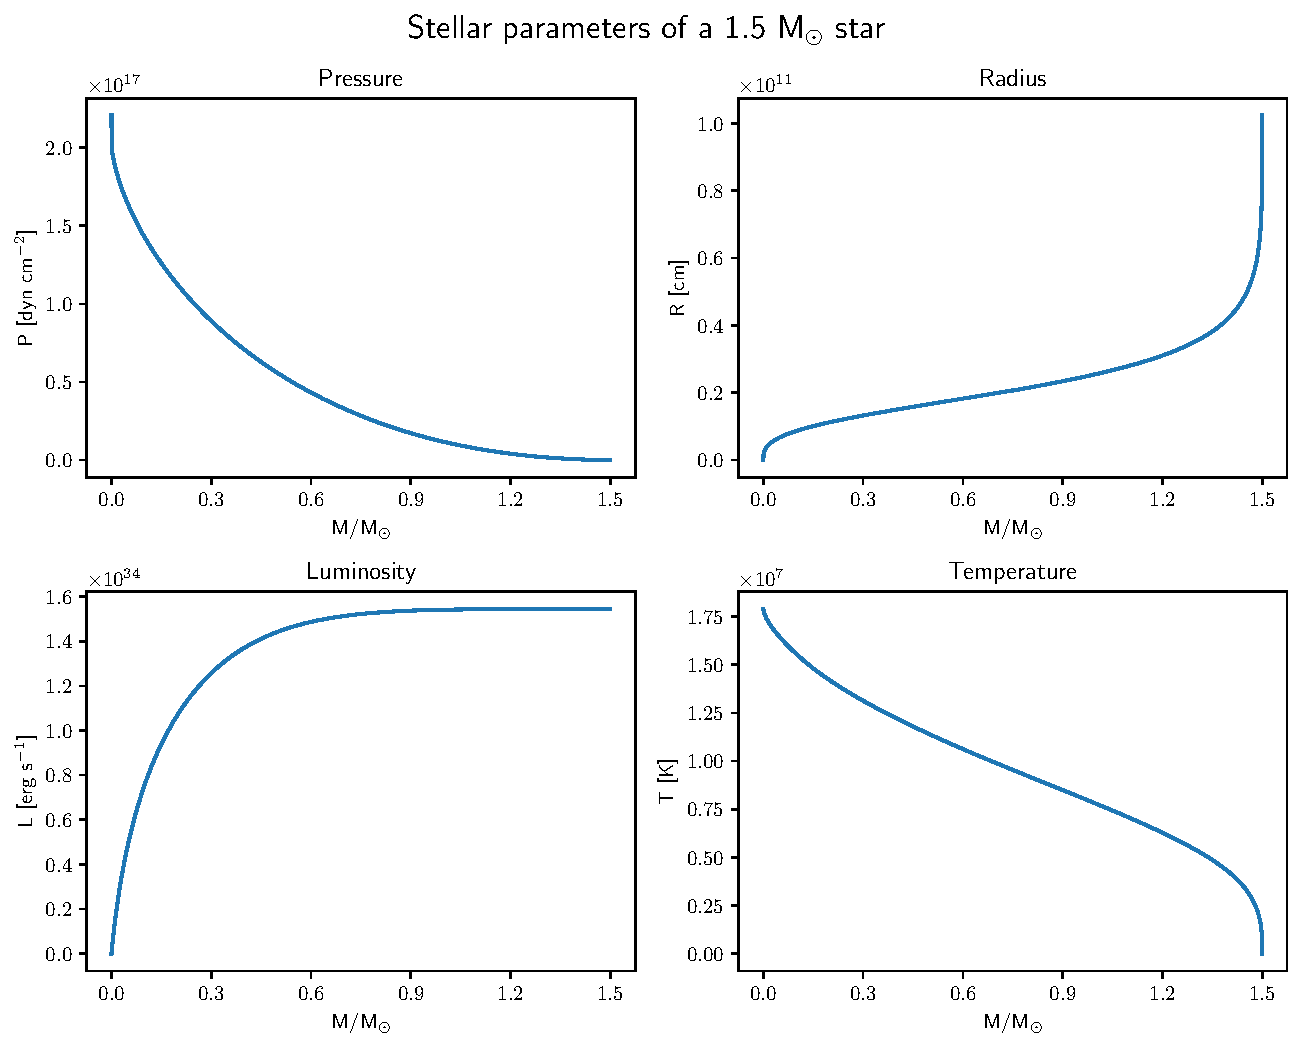
\includegraphics[scale=0.8]{figures/4plots.pdf}
% 	\caption{Pressure, radius, luminosity, and temperature within the star of 1.5M$_\odot$ with solar compositions calculated using the method describe in this report.}
% 	\label{fig:main_4plots}
% \end{figure*}
\begin{figure*}
	\centering
	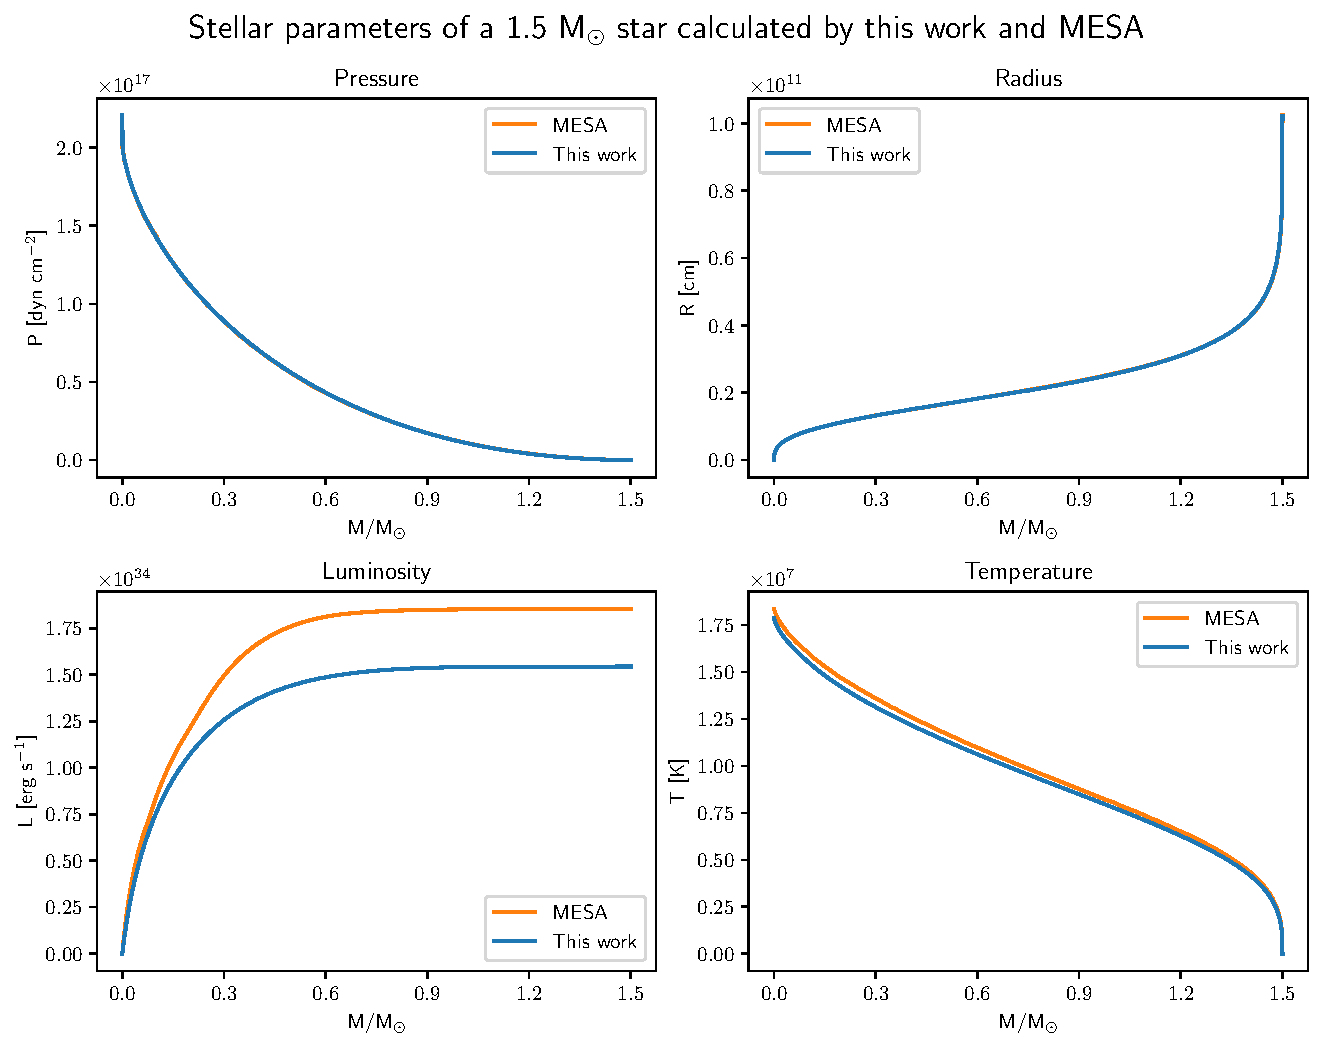
\includegraphics[scale=0.66]{figures/4plots_mesa.pdf}
	\caption{Pressure, radius, luminosity, and temperature within the star of 1.5M$_\odot$ with solar compositions calculated using the method describe in this report and MESA the state of art stellar evolution code. Note that for pressure and radius, two plots on top of each other.}
	\label{fig:main_4plots_mesa}
\end{figure*}

\begin{table}[ht!]
	\centering
	\begin{tabular}{|c|c|c|}
		\hline
		            & Value                                     & residue in  ppm \\ \hline
		$P_c$    & \num{2.206e17} $\mathrm{dyn ~ cm^{-3}}$ & 1.8418                                                           \\ \hline
		$R$      & \num{1.023e+11} $\mathrm{cm}$           & 1.4703                                                           \\ \hline
		$\mathcal{L}$  & \num{1.544e+34} $\mathrm{erg ~ s^{-1}}$ & 1.6426                                                           \\ \hline
		$T_c$ & \num{1.789e7} $\mathrm{K}$              & 0.4529                                                           \\ \hline
	\end{tabular}
	\caption{Best fit stellar parameters (Central pressure, radius, luminosity and central temperature) and the normalised remaining residue at the fitting point in parts per million}
	\label{tab:final_results}
\end{table}









\section{Comparison with MESA}
\label{sec:mesa}
Modules for Experiments in Stellar Astrophysics (MESA) (\cite{MESA}) is a state of an art stellar evolution code. To evaluate the accuracy of the numerical calculation in this report, the results obtained in this work are compared with the MESA model and they are shown in Figure \ref{fig:main_4plots_mesa} and Table \ref{tab:mesa_results}. It can be seen from the table that for radius and temperature, the results are very close. However, for central pressure and the star's luminosity, the results are off by 9.45\% and 17.2\% respectively. Considering the simplicity of the model used in this report, the results are very satisfactory. The overall shape of the parameters within the star matches very well with the MESA model as shown in Figure \ref{fig:main_4plots_mesa}.

\begin{table*}[htb!]
	\centering
	\begin{tabular}{|c|c|c|c|}
		\hline
		                                     & This work         & MESA               & Percentage difference \\ \hline

		Central Pressure ($\mathrm{dyn ~ cm^{-3}}$)  & \num{2.206e+17}  & \num{2.015e+17}  & 9.45\%                \\ \hline
		Radius ($\mathrm{cm}$)               & \num{1.023e+11} & \num{ 1.023e+11} & 0.00348\%             \\ \hline
		Luminosity ($\mathrm{erg ~ s^{-1}}$) & \num{1.544e+34} & \num{1.865e+34}  & -17.2   \%            \\ \hline
		Central Temperature ($\mathrm{K}$)           & \num{1.789e7}   & \num{1.836e+7}  & -2.57  \%             \\ \hline
	\end{tabular}
	\caption{Comparison of the results of this work and the MESA model}
	\label{tab:mesa_results}
\end{table*}

% \begin{deluxetable*}{|c||c|c|c|c|}[ht]
% 	\tablecaption{Comparison of the results of this work and the MESA model}
% 	\label{tab:results_mesa2}
% 	\tabletypesize{\scriptsize}
% 	\tablehead{
% 		\colhead{} & \colhead{Pressure ($\mathrm{dyn cm^{-3}}$)} &\colhead{Radius ($\mathrm{cm}$)} &\colhead{Luminosity ($\mathrm{erg ~ s^{-1}}$)} & \colhead{Temperature ($\mathrm{K}$)}
% 	}
% 	\startdata
% 	This work  & 2.20589e+17 & 1.02301e+11 & 1.54274e+34 & 1.78849e+07 \\ \hline
% 	MESA       & 2.01526e+17 & 1.02312e+11 & 1.86454e+34 & 1.83587e+07 \\ \hline
% 	Difference & 9.46\%         & -0.0115\%      & -17.3\%        & -2.58\%        \\ \hline
% 	\enddata
% \end{deluxetable*}

\section{Source code}
The source code of this work, machine-readable table of the results are available at \url{https://github.com/zoutei/JHU_stellar_project}.

\section{Conclusion}
\label{sec:conclusion}
In this report, the structure of a zero-age main sequence star of 1.5M$_\odot$ with solar compositions ($X = 0.70, ~Y = 0.28, ~Z = 0.02$) is modelled by numerically integrating four coupled differential equations. Equations assume the star, which is made out of fully ionised ideal gas, is in hydrostatic equilibrium where the pressure gradient, which is the sum of ideal gas pressure and the radiation pressure, is balanced by gravitational force. The energy generation rate is calculated using the pp chain and CNO cycle. The energy in the star is transported by either radiation or convection. The opacity is interpolated from the tabular data provided by the OP project. The boundary conditions are set at the centre and the surface. The inner boundary is at a small distance away from the centre where $\mathcal{M}_{r, {c^\prime}} = 1 \times 10^{-5} ~ \mathcal{M}$. The outer boundary is defined at the star's photosphere where the optical depth $\tau$ is 2/3.

The numerical calculation is conducted using the Runge-Kutta method of order 4 with an error estimator of order 5 (RK45) from the centre and the surface to the intermediate fitting point, which is known as the shooting method. To find the best stellar parameters that satisfy both boundary conditions, the residues at the fitting point are minimised using the \verb|L-BFGS-B| algorithm with 16 iterations starting from appropriate initial guesses.

The results shows such star to have the central pressure $P_c = $ \num{2.206e17} $\mathrm{dyn ~ cm^{-3}}$, radius $\mathrm{R} = 1.470 \mathrm{R}_\odot$, luminosity $\mathcal{L} = 4.036  \mathrm{L}_\odot$ and central temperature $T_c = $ \num{1.789e7} $\mathrm{K}$ . These results are compared with the state-of-the-art MESA model and it is found that the results are very close for radius and central temperature with the difference of 0.004 \% and 2.57 \% respectively. However, for central pressure and the star's luminosity, the results are off by 9.45\% and 17.2\% respectively. Considering the simplicity of the model used in this report, the results are very satisfactory. The overall shape of the parameters within the star matches very well with the MESA model.

\bibliography{refs}{}
\bibliographystyle{aasjournal}
\nocite{*}

\end{document}
